\documentclass[../Hovedrapport.tex]{subfiles}
\begin{document}
%\vspace{-30pt}
%------------------------------------------------------------------------------
\section{Kontrol af fordamperydelse (J.K. \& C.R.)}
    \label{sec:dim_fordamper}
I følgende afsnit vil en udvalgt fordamper blive gennemregnet med henblik på at bestemme dens potentielle kuldeydelse. Gennem en iterativ proces er fordamperstørrelsen blevet udvalgt således, at den lever op til kravet om en maksimal kuldeydelse på \SI{334}{W} ved et omdrejningstal på \SI{4000}{RPM} (Jf. tabel \ref{tab:kompressor_Data}). Omend fordamperen er en lamelvarmeveksler, vil den blive betragtet som et ribberørsbundt for at muliggøre beregningerne i afsnittet. Dette skyldes, at det udvendige varmeovergangstal er meget vanskeligt at beregne på lamelvarmevekslere.

\subsection{Dimensioner af fordamper  (J.K. \& C.R.)}
På nedenstående skitser ses varmeveksleren, hvor de relevante dimensioner er angivet med navngivning, som vil blive benyttet til udregningerne.

% Dimension 1 
\begin{figure}[H]
    \centering    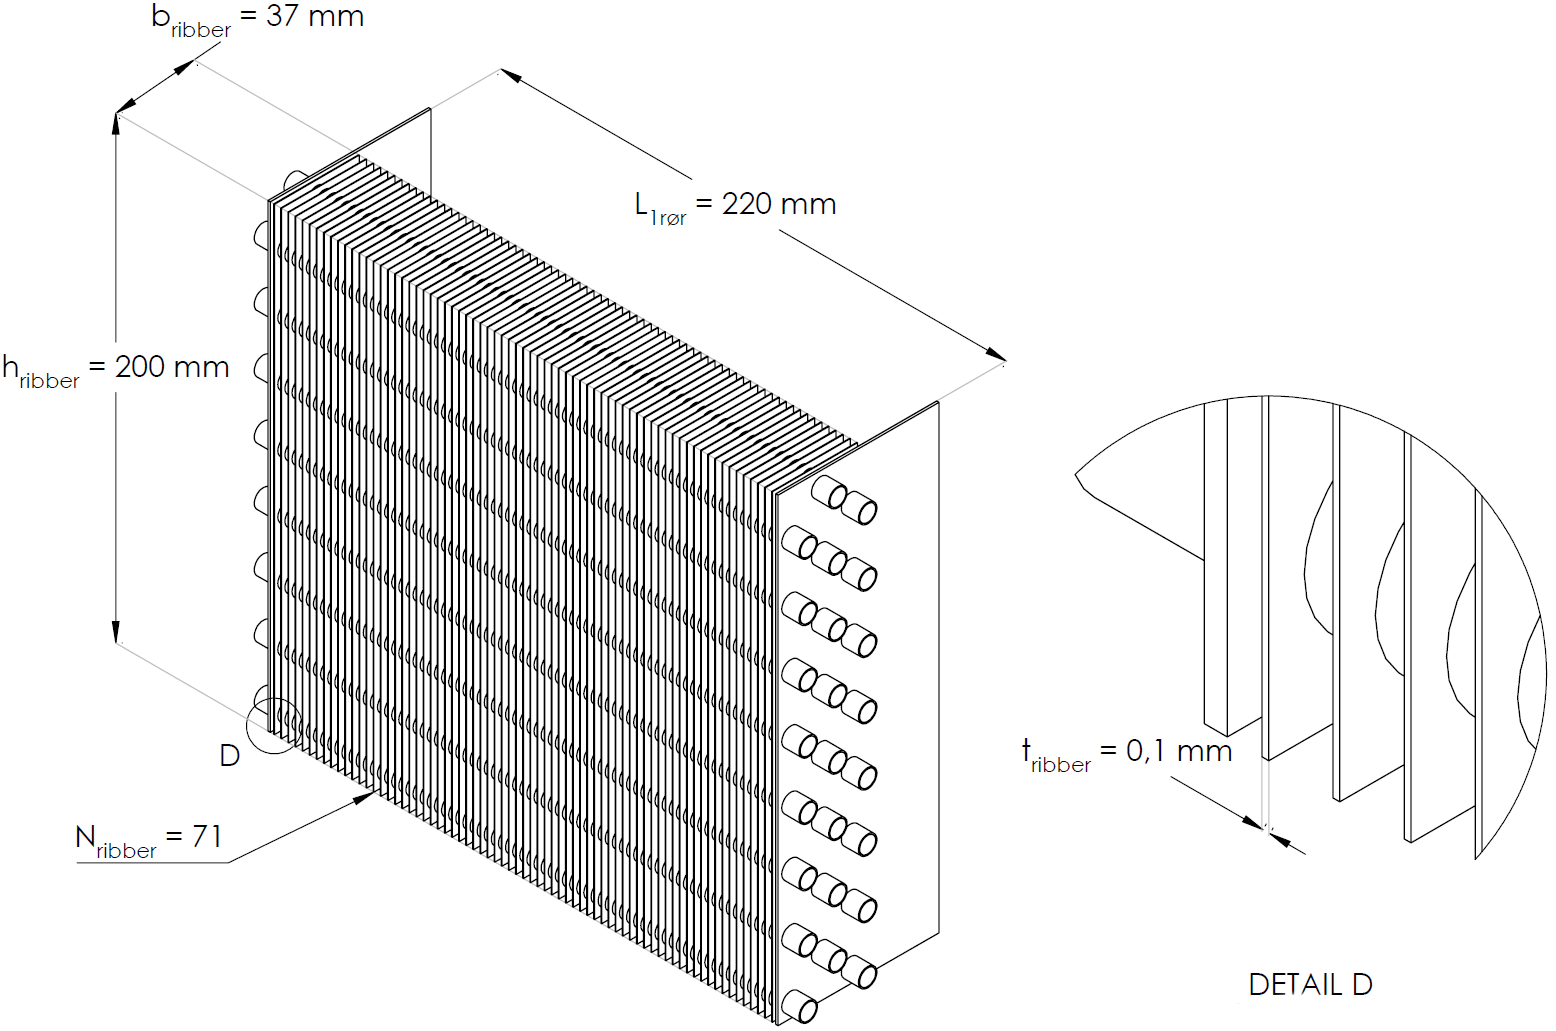
\includegraphics[width=0.9\textwidth]{Billeder/varmevekslerdim1.png}
    \caption{\textit{Dimensioner på varmeveksler}.}
    \label{fig:varmevekslerdim1}
\end{figure}
% Dimension 2 
\begin{figure}[H]
    \centering
    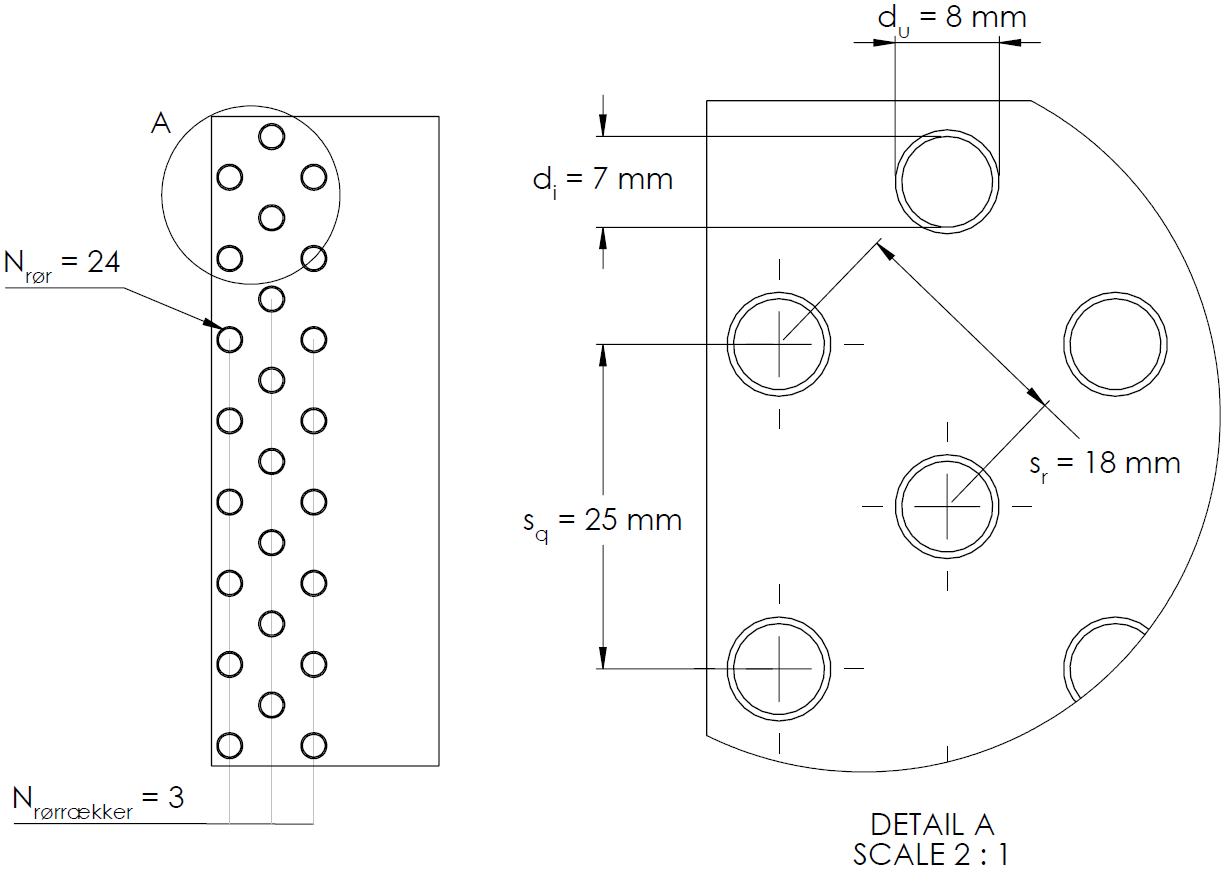
\includegraphics[width=0.8\textwidth]{Billeder/varmevekslerdim2.png}
    \caption{\textit{Dimensioner på varmeveksler - fortsat}.}
    \label{fig:varmevekslerdim2}
\end{figure}


\subsubsection*{Anlægsdata}
I den nedenstående tabel \ref{tab:Fordamper_anlægs_Data} fremgår det, hvilke omstændigheder fordamperen er beregnet under. Tabellen har til formål at overskueliggøre værdier af de antagelser, der er gjort. I tabellen fremgår betegnelser med dertilhørende indeks, som benyttes i beregningerne i dette afsnit \ref{sec:dim_fordamper}.

\begin{table}[H] 
	\centering
	% \caption*{\textbf{\large Fordamper data}} 
	% \vspace{-0.3cm}
	\begin{tabular}{|c|c|c|c|}  \rowcolor[gray]{0.7}                                \hline
	\multicolumn{4}{|c|}{\textbf{Anlægsdata}}                                                   \\ \hline \rowcolor[gray]{.8}
	\textbf{Betegnelse}   & \textbf{Værdi}        & \textbf{Forklaring}       & \textbf{Kilde}    \\ \hline \
	x_\text{g}          & 1                     & Dampkvalitet - mættet væske   & \\ \hline 
	x_\text{l}          & 0                     & Dampkvalitet - mættet gas & \\ \hline

%	C                   & 0,41                  & Faktor c for fortsatte røranordning         & Aages noter \\ \hline \rowcolor[gray]{.95}   
%	m                   & 0,60                  & Eksponent M for fortsatte røranordning      & Aages noter     \\ \hline \rowcolor[gray]{.95}
	t_\text{f}         & \SI{-8}{\celsius}     & Fordampningstemperaturen                   & Antagelse       \\ \hline 
	t_\text{a}        & \SI{7}{\celsius}      & Lufttemperaturen før fordamperen              & Antagelse     \\ \hline
	t_\text{b}        & \SI{4}{\celsius}      & Lufttemperaturen efter fordamperen            & Gæt     \\ \hline 
%     t_\text{R1}         & \SI{-8}{\celsius}     & Kølemiddlets temperatur før fordamperen        & Antagelse    \\ \hline 
% 	t_\text{R1}         & \SI{-8}{\celsius}     & Kølemiddlets temperatur efter fordamperen        & Antagelse  \\ \hline 
    c_\text{L}         & \SI{3}{\frac{m}{s}}     & Lufthastigheden over fordamperen        & Målt  \\ \hline
    q_\text{mR}         & 2,43 \cdot 10^{-3} \SI{}{\frac{kg}{s}}    & Massestrøm af kølemiddel gennem fordamperen        & Afsnit \ref{sec:masse}  \\ \hline 
	\end{tabular} 
	\caption{\textit{Anlægsdata for fordamperen}} 
	\label{tab:Fordamper_anlægs_Data} 
	\vspace{-20pt}
\end{table}
% Vi bør overveje om temperaturen ikke skal estimere til 4 degC fordi det er nermere den man vil have i et køleskab. jo men så skal der jo ikke køles noget ned.
Det vil ikke være nødvendigt for kompressoren at køre med maksimale omdrejninger, hvis der er omkring \SI{4}{\celsius} inde i køleskabet. Det antages, at \SI{7}{\celsius} er den laveste lufttemperatur i køleskabet, hvor kompressoren stadigvæk kører med \SI{4000}{RPM}, hvilket vil afhænge af den senere programmering. 

Luftens temperatur falder ved passage igennem fordamperen og i første omgang gættes en værdi for luftens udgangstemperatur. Denne temperatur gættes indledningsvist til $\SI{4}{\celsius}$. Til slut vil der gennem en iterativ proces blive bestemt en mere nøjagtig værdi for afgangstemperaturen, ud fra den beregnede kuldeydelse.

Det antages desuden, at kølemiddlet har en konstant temperatur igennem fordamperen, hvilket svarer til fordampningstemperaturen på $\SI{-8}{\celsius}$. Her ses der bort fra overhedningen på $\SI{8}{\kelvin}$, da indflydelsen heraf antages at være negligibel og yderligere vil komplicere udregningerne.
\begin{align}
    t_{2}= t_{1} = \SI{-8}{\celsius}   
\end{align}
Af nedenstående figurer fremgår temperaturforløbet for luften og kølemiddelt igennem fordamperen. 
\begin{figure}[H]
	\centering
	\begin{minipage}[b]{0.495\textwidth}
	\centering
	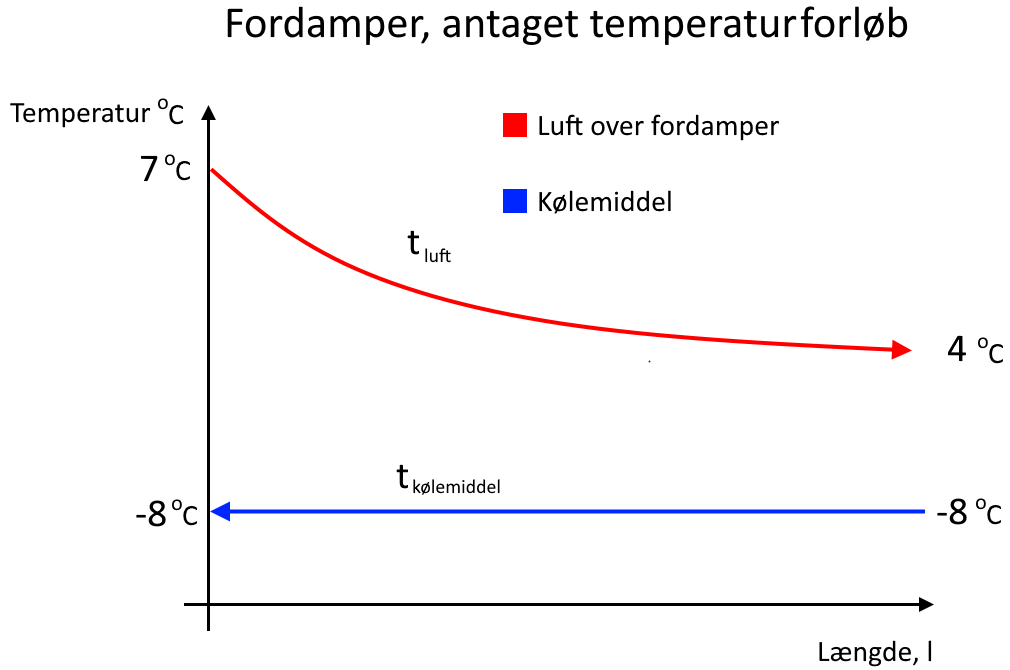
\includegraphics[width=1.00\textwidth]{Billeder/temp_fordamp.png} % Venstre billede
	\end{minipage}
	\hfill
	\begin{minipage}[b]{0.495\textwidth}
	\centering
	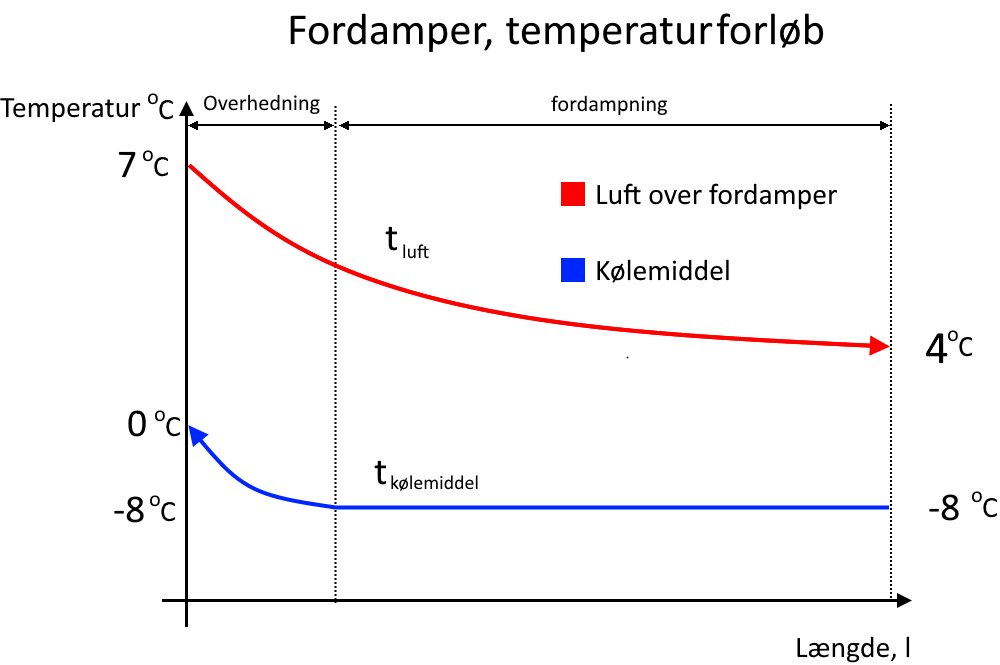
\includegraphics[width=1.00\textwidth]{Billeder/reel_tf_ny.png} % Højre billede
	\end{minipage}
	\\ % Figurtekster og labels
	\begin{minipage}[t]{0.45\textwidth}
	\caption{\textit{Antaget temperaturforløb i fordamper}.} % Venstre figurtekst og label
	\label{fig:Temperaturforloeb_fordamper}
	\end{minipage}
	\hfill
	\begin{minipage}[t]{0.45\textwidth}
	\caption{\textit{Reel temperaturforløb i fordamper}.} % Højre figurtekst og label
	\label{fig: Reel temperaturforløb igennem fordamper med overhedning.}
	\end{minipage}
\end{figure}
Disse antagelser medfører en middeltemperatur for luften gennem fordamperen på:
\begin{align}
    t_{Lm}= \dfrac{t_{a}+t_{b}}{2} = \SI{5,5}{\celsius} % bedst at skrive den i celsius, da både tl1 og tl2 er i celsius
\end{align}
Slutteligt sidder der en blæser og laver tvungen luftstrømning igennem fordamperen. Blæserne for denne størrelse fordamper har én grundindstilling, hvorpå lufthastigheden er målt til $c_{\textit{{L}}}= \SI{3}{m/s}$. Hertil antages det, at trykket er $p_{\textit{{L}}}= \SI{1}{bar}$.

% --- Beregning af den totale varmeovergangsmodstand ---

\subsection{Beregning af den totale termiske modstand  (J.K. \& C.R.)}
    \label{sec:Beregning_af_den_totale_varmeovergangsmodstand1}

% Venstre søjle
\begin{minipage}[t]{0.58\textwidth}
For at  bestemme kuldeydelsen, $\si{\Phi_0}$, som fordamperen leverer, og varmegennemgangstallet, U, skal den totale termiske modstand, som varmestrømmen møder fra luften til kølemidlet igennem fordamperens rør, kendes. Modstanden består af en varmeovergangsmodstand fra luften til aluminiummet på rør og ribber. Rørene er lavet af kobber belagt med et tyndt lag aluminium. Qua den minimale tykkelse af aluminiummet betragtes rørene som værende kobberrør. På figur \ref{fig:modstande_i_roer} ses de termiske modstande, som varmen møder igennem røret til kølemiddlet. $R_{OU}$ og $R_{OI}$ er varmeovergangsmodstande og $R_{\text{rør}}$ er varmeledningsmodstanden. Fordamperen antages at være fri for smuds og skidt. Derfor bidrager dette ikke til en yderlig termisk modstand.
\end{minipage} \hfill
% Højre søjle:
\begin{minipage}[t]{0.4\textwidth}
\begin{figure}[H]
    \centering
   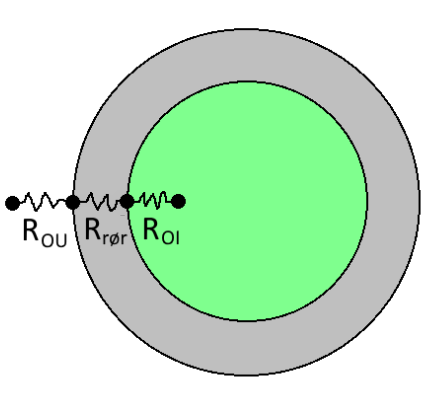
\includegraphics[width=0.8\textwidth]{Billeder/Modstande.png}
    \caption{\textit{Her ses de samlede modstande ved varmetransmissionen igennem rør}.}
    \label{fig:modstande_i_roer}
\end{figure}
\end{minipage}

%%
%	\begin{minipage}[t]{0.4\textwidth}
%	\begin{figure}[H]
%	\centering
%	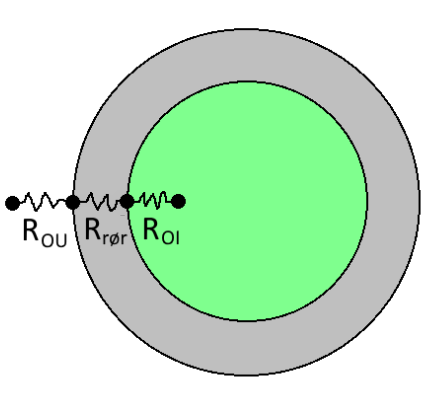
\includegraphics[width=1.00\textwidth]{Billeder/Modstande.png} % Venstre billede
%	\end{figure}
%	\end{minipage}
%	\begin{minipage}[t]{0.35\textwidth}
%	\caption{\textit{Her ses de samlede modstande ved varmetransmissionen igennem rør}.} % Venstre figurtekst og label
%	\label{fig:modstande_i_roer}
%	\end{minipage}
%%
\subsection{Beregning af det udvendige varmeovergangstal og overgangsmodstand, $\alpha_\text{ou}$ og $R_\text{ou}$  (J.K. \& C.R.)}
    \label{sec:Udvendig_varmeovergangsmodstand_fordamper}
Den udvendige varmeovergangsmodstand imellem luften og aluminiumbelægningen skal bestemmes. Hertil findes Nusselts tal udvendigt på rørene og ribberne. Til at bestemme Nusselts tal skal Reynolds tal og Prandlts tal udvendigt på fordamperen kendes. 

Nusselts tal bestemmes med nedenstående formel, hvorefter denne bruges til at bestemme varmeovergangstallet $\alpha_\text{ou}$ med den generelle formel for Nusselts tal \citep{Noter_Aage}. 
\begin{equation}
    \si{Nu_u}  = C \cdot   \left( \V{Re} _{u} \right) ^{m} \cdot   \left(\frac{A_{t}}{A_{0}} \right) ^{m-1}    \cdot  \V{{Pr} _{u}}^{0,33}
\end{equation}
Først findes det udvendige Reynoldstal, dertil findes den kinematiske viskositet i \textit{EES} ved middeltemperaturen $t_{Lm} = \SI{5,5}{\celsius}$ for luften og trykket i luften på $\SI{1}{\bar}$.
\begin{equation}
\si{\nu_L} = 14,0\cdot 10^{-6}\si{\frac{m^2}{s}}
\end{equation}
Reynolds tal beregnes ud fra hastigheden af luften gennem fordamperen over den ydre diameter af de tværgående rør med nedstående formel \citep{termo}.
\begin{equation}
\V{Re} _{u} =\frac{c_{L} \cdot  d_{u}}{\si{\nu}} = 1720
\end{equation}
Her ses det, at der er tale om laminar strømning på tværs af rørene, da værdien er under $ 2 \cdot 10^{5} $ \citep{termo}. Ved samme middeltemperatur og tryk som den kinematiske viskositet bestemmes Prandtls Tal for den udvendige del af fordamperen i \textit{EES}:
\begin{equation}
Pr_{u} = 0,71		 
\end{equation}
Det totale overfladeareal af rør og lameller i fordamperen skal beregnes. Arealet af rørstykkerne mellem lameller er:
\begin{equation}
A_{0} = d_{u} \cdot  \pi \cdot  L_{\text{rør}} -  \left( d_{u} \cdot  \pi \cdot  t _{ribber} \cdot  N_{ribber} \right) = \si{0,133}{m^2}	 
\label{eq: Areal af rørstykker mellem ribber}
\end{equation}
Det totale areal af fordamperen bliver dermed:
\begin{equation}
A_{t} = A_{0} +  \left( b_{ribber}\cdot N_{serie}\cdot h_{ribber} -  \left(\frac{d_{u}}{2}\right) ^{2}\cdot \pi\cdot N_{\text{rør}} \right) \cdot 2\cdot N_{ribber	} = \SI{1,01}{m^2}	
\label{eq: Total overfladeareal fordamper}
\end{equation}
Fra \citep{Grundlagen_der_Wärmeübertragung} kommer nedstående tabel. Her slås værdier for C og m op afhængigt af, hvilken type fordamper der benyttes. Den valgte fordamper har tre rørrækker, som er forsatte over for hinanden. Derfor bliver værdierne for C og m for den beregnede fordamper C = 0,41 og m = 0,60.
  \begin{table}[H]
    \centering
    \begin{tabular}{|c|c|c|c|c|c|} \hline \rowcolor[gray]{.7}
    \multicolumn{6}{|c|}{Værdier for C og m ud fra rørrækkeantal}              \\ \hline \rowcolor[gray]{.8}
    \multicolumn{2}{|c|}{Ribberørrækker} & 1  & 2  & 3  & >=4       \\ \hline
    \multirow{2}{*}{Flugtende} & m  & 0,53 & 0,61  & 0,67  & 0,68   \\ \cline{2-6}
     & C  & 0,37  & 0,295  & 0,22  & 0,1                            \\  \hline
    \multirow{2}{*}{Forsatte} & m  & 0,53  & 0,56  & \cellcolor{green!25} 0,60  & 0,63   \\ \cline{2-6}
     & C  & 0,37  & 0,39  & \cellcolor{green!25} 0,41 & 0,43                             \\ \hline
    \end{tabular}
    \caption{\textit{Tabel med værdier for C og m fra \citep{Danvak}}}
    \label{tab:c_og_M}
    \end{table}

Nu kan det udvendige Nusselts tal beregnes:
\begin{equation}
    \si{Nu_u}  = C \cdot   \left( \V{Re} _{u} \right) ^{m} \cdot   \left(\frac{A_{t}}{A_{0}} \right) ^{m-1}    \cdot  \V{Pr} _{u}^{0,33} = 14,2
\end{equation}




% -------------------- Det udvendige varmeovergangstal -------------------

Ved brugen af den generelle formel for Nusselts tal kan varmeovergangstallet beregnes:

\begin{equation}
    \V{Nu_u}  = \frac{\alpha_{u} \cdot  d_{u}}{\lambda_{L}}
\end{equation}


Varmekonduktiviteten for luft slås op i \textit{EES} ved middeltemperaturen for luft ved et tryk på 1 bar.

\begin{equation}
    \si{\lambda_{L}} = \SI{0,0248}{\frac{W}{m\cdot K}}
\end{equation}

Ved de ovenstående værdier kan det udvendige varmeovergangstal for rørene regnes til følgende:

\begin{equation}
    \alpha_\text{ou} = \frac{\V{Nu_u} \cdot \lambda_{L}}{d_{u}} = \SI{43,9}{\frac{W}{m^2 \cdot K}}
\end{equation}



% -------------------- Ribbeevirkningsgrad ----------------------------
\subsubsection*{Ribbevirkningsgrad}
    \label{sec:ribbevirkningsgrad}
For at beregne den udvendige varmeovergangsmodstand bestemmes varmevekslerens ribbevirkningsgrad. Dette foretages i henhold til proceduren i \citep{Danvak} kapitel 14. Idet lamelvarmeveksleren antages at være et ribberørsbundt bestemmes ribbehøjden $ l_{ribber} $. Heri indgår konstanterne $s_q = \SI{0,025}{m}$ og $s_r = \SI{0,018}{m}$, som fremgår af figur \ref{fig:varmevekslerdim2}:
\begin{align}
\lambda_{ribber} &  &&=\SI{233}{\frac{\watt}{m \cdot K}} &&\text{$\lambda_{ribber}$, opslag i EES (aluminium)} \\
l_{ribber} &= \frac{s_q}{2}-\frac{d_u}{2} &&=\SI{0,0085}{m} &&\text{Ribbehøjden - Danvak figur 14.10} \\
L &= l_{ribber} \cdot \sqrt{\frac{2 \cdot \alpha_u}{\lambda_{ribber} \cdot t_{ribber}}} &&= 0,521 &&\text{L - Danvak ligning 14.7} \\
\beta &= 1,27 \cdot \sqrt{\frac{\frac{s_r}{2}}{\frac{s_q}{2}}-0,3} &&= 0,823 &&\text{\beta, forsatte rør, Danvak ligning 14.10}\\
\Psi &= 1+0,35 \cdot \beta \cdot \ln{\frac{\frac{s_q}{2}}{\frac{d_u}{2}}} &&= 1,33 &&\text{\Psi, enhedsløs - Danvak ligning 14.10}
\end{align}
Hernæst beregnes ribbevirkningsgraden, som tager hensyn til temperaturændring over en ribbe. Dette benyttes til at bestemme den udvendige varmeovergangsmodstand:
\begin{align}
\eta_{ribber} = \frac{\tanh{(L \cdot \Psi)}}{L \cdot \Psi} = 0,866 &&\text{Danvak ligning 14.9}
\end{align}

% ------ Resultat er udvendig varmeovergangsmodstand ----

Nu kan den udvendige varmeovergangsmodstand bestemmes:
\begin{equation}
R_{ou} = \frac {1}{  \left( \alpha_{u} \cdot  A_{t} \cdot  \eta_{ribber} \right)  } = \SI{0,0260}{\frac{K}{W}}
\end{equation}
Det fremgår heraf, at den udvendige varmeovergangsmodstand er på $\SI{0,026}{\frac{K}{W}}$.

% Det ovenstående er et meget stort tal. Hvor er arealet udregnet!=!!)!=P!=!?


% ---------- Varme gennemgangsmodstand --------------------

\subsection{Beregning af varmeledningsmodstanden, $R_\text{rør}$  (J.K. \& C.R.)}
    \label{sec:Varmeledningsmodstand}

Kobberrørene som kølemidlet løber i har en varmeledningsmodstand. Denne modstand er materialespecifik og beregnes for rørvæggen ${R_{\textit{rør}}}$. Dette gøres med formlen for varmeledningsmodstand i en rørvæg.

Varmekonduktiviteten før røret slås op i \textit{EES} for kobber ved temperaturen -8 $\si{\celsius}$.
\begin{equation}
\lambda_\text{rør} = \SI{400}{\frac{W}{m \cdot K}}
\end{equation}
Varmeledningsmodstanden igennem rørvæggen beregnes:
\begin{equation}
R_\text{rør} = \frac {\ln{ \left( \frac{d_{u}}{d_{i}} \right) }}{  \lambda_{\text{rør}} \cdot  2 \cdot  \pi \cdot  L_{\text{rør}}} =10,1\cdot 10^{-6}\si{\frac{K}{W}}
\end{equation}



% --- Nu beregnes den indvendige varmeovergangsmodstand ---

\subsection{Beregning af det indvendige varmeovergangstal og overgangsmodstand, $\alpha_\text{oi}$ og $R_\text{oi}$  (J.K. \& C.R.)}
    \label{sec:Indvendig varmeovergangsmodstand}

Den indvendige varmeovergangsmodstand fra rørene til kølemidlet beregnes med Bo Pierres metode \citep{koleteknik}. Først findes Nusselts tal, som bruges til at beregne det indvendige varmeovergangstal, via den generelle formel for Nusselts tal. Det antages, at der er tale om tør operation, idet systemet styres med en temperaturstyret ekspansionsventil. 

Formlen for Nusselts tal ved tør operation er jf. Bo Pierres metode:
\begin{equation}
\V{Nu_i}  = 0,0075 \cdot   \left( \V{{Re} _{i}}^{2} \cdot  K_{f} \right) ^{0,4}
\end{equation}
Reynolds tal beregnes ligeledes efter Bo Pierres metode \citep{koleteknik}:
\begin{equation}
\V{Re} _{i} = \frac{q_{mR} \cdot d_{i}}{ S_{i} \cdot  \eta_{l}}
\end{equation}
Den dynamiske viskositet for kølemidlet slås op i \textit{EES} ved fordampningstemperaturen på $\SI{-8}{\celsius}$ og mættet væsketilstand  jf. Bo Pierres metode. Derfor sættes dampkvaliteten,\textit{x}, lig med 0.
\begin{equation}
\si{\eta_{l}} =295\cdot 10^{-6} \SI{}{\frac{kg}{m \cdot s}}
\end{equation}
Rørets indvendige tværsnitsareal i fordamperen er:
\begin{equation}
S_{i} = \frac{\pi}{4}\cdot  d_{i}^{2} = 38,5\cdot 10^{-6}\SI{}{m^2}
\end{equation}
Reynolds tal kan hernæst beregnes:
\begin{equation}
\V{Re} _{i} = \frac{q_{mR} \cdot d_{i}}{ S_{i} \cdot  \eta_{l}} = 1500
\end{equation}
Nu bestemmes Kogtallet med formlen:
\begin{equation}    
K_{f} = \frac {r}{ L_{\text{rør}}\cdot g}
\end{equation}
Fordampningsentalpien for kølemidlet slås op i \textit{EES} ligeledes ved \SI{-8}{\celsius}.
\begin{equation}
r = \SI{205}{\frac{kJ}{kg}} 
\end{equation}
Kogtallet beregnes nu for kølemidlet. Det gøres med nedenstående formel:
\begin{equation}    
K_{f} = \frac {r}{ L_{\text{rør}}\cdot g} = 3950
\end{equation}
Nu kan Nusselts tal for den indvendige del af røret findes:
\begin{equation}
\V{Nu_i}  = 0,0075 \cdot   \left( \V{Re} _{i}^{2} \cdot  K_{f} \right) ^{0,4} = 71,6
\end{equation}
Ud fra Nusselts tal kan varmeovergangstallet bestemmes med formlen:
\begin{equation}
    \V{Nu_i}  = \frac{\alpha_{u} \cdot  d_{u}}{\lambda_{Ri}}
\end{equation}
Varmekonduktiviten for kølemidlet i mættet væsketilstand slås op i \textit{EES};
\begin{align}
\lambda_{Ri} &= \SI{0,0980}{\frac{W}{m \cdot K}}
\end{align}
Det indvendige varmeovergangstal bestemmes nu: 
\begin{align}
\alpha_\text{oi} &= \frac{{Nui} \cdot \si{\lambda_{Ri}}}{d_{i}} = \SI{1000}{\frac{\watt}{m^2 \cdot K}}
\end{align}
Nu kan varmeovergangsmodstanden indvendigt i rørene, $R_{oi}$, beregnes ved tvungen konvektion indvendigt i rør \citep{termo} formel 9.23:
\begin{equation}
R_{oi} = \frac {1}{\alpha_{i} \cdot  A_{i}} 
\end{equation}
Overfladeareal indvendigt på rørene:
\begin{equation}
A_{i} = d_{i} \cdot  \pi \cdot  L_{\text{rør}} = \SI{0,116}{m^2}
\end{equation}
Slutteligt kan den indvendige varmeovergangsmodstand bestemmes:
\begin{equation}
R_{oi} = \frac {1}{\alpha_{i} \cdot  A_{i}} = \si{0,00860}{\frac{K}{W}}
\end{equation}

% ------- Total varmeovergangsmodstand ----------
\subsection{Beregning af total varmegennemgangsmodstand  (N.J. \& M.N.)}
    \label{sec:VarmeledningsmodstandF}
Nu beregnes den totale termiske modstand, $R_\text{total}$, varmen oplever, når den går fra luften gennem rørvæggen og til kølemidlet i fordamperen. Dette gøres ved at addere de tre termiske modstande. Dermed bliver den totale varmeovergangsmodstand fra luft til væske:
\begin{equation}
R_\text{total} = R_{ou} + R_{oi} + R_\text{rør} = \si{0,0346}{\frac{K}{W}} 	
\end{equation}
% ---- Beregning af den logaritmiske middeltemperatur differens ----
\subsection{Beregning af den logaritmiske middeltemperaturdifferens  (J.K. \& C.R.)}
    \label{sec:Massestrøm af kølemiddel}
Den logaritmiske middeltemperaturdifferens, $\si{\Delta{t_m}}$, beregnes med formlen nedenfor. Denne skal bruges til at beregne varmegennemgangstallet og kuldeydelsen, som fordamperen yder \citep{koleteknik}. Her antages det, at temperaturen på kølemidlet er konstant igennem hele fordamperen, og at denne har temperaturen $\SI{-8}{\celsius}$. Luftens temperatur før og efter fordamperen er henholdsvis $\SI{7}{\celsius}$ og $\SI{4}{\celsius}$. Den logaritmiske middeltemperaturdifferen beregnes ud fra temperaturforløbet, som fremgår af figur \ref{fig:Temperaturforloeb_fordamper} 

\begin{align}
\Delta t_{m} = \frac{(t_{a}-t_{2})-(t_{b}-t_{1})}{\text{ln}{ \left( \frac{t_{a}-t_{2}}{t_{b}-t_{1}} \right) }} = \SI{13,4}{\kelvin}
\end{align}
På fordamperen bruges der, som førnævnt, en blæser til at tvinge en luftstrøm på $3 \frac{m}{s}$ mellem lameller og tværs over rørene. Dette kan betragtes som en krydsstrøm over rørene, idet luften blæser tværs over disse. Til at korrigere den logaritmisk middeltemperaturdifferens bruges korrektionsfaktoren $\epsilon$. 
Den logaritmiske middeltemperaturdifferens er beregnet som en modstrøm, men multipliceres med en korrektionsfaktor for kydsstrøm. Korrektionsfaktoren for denne er \citep{koleteknik}:
\begin{align}
    \epsilon &= 1   
\end{align}
Således bliver middeltemperaturdifferensen med korrektion for krydsstrøm
\begin{align}
   \Delta{t_{mkryds}} &= \si{\epsilon}\cdot\si{\Delta{t_m}} = \SI{13,4}{\kelvin}
\end{align}

\subsection{Beregning af kuldeydelse og varmegennemgangstal  (J.K. \& C.R.)}
Idet $R_\text{total}$ og $\Delta t_{mkryds}$ kendes, kan kuldeydelsen, $\Phi_v$, og varmegennemgangstallet, U, bestemmes. Kuldeydelsen for fordamperen er den mængde energi, som kan optages under de beregnede testforhold. Denne er:
\begin{equation}
\Phi_{0} = \frac {{\Delta t}_{mkryds}}{R_\text{total}} = \SI{388}{W}
\end{equation}
Varmegennemgangstallet for fordamperen beregnes herefter til:
\begin{equation}
U_u = \frac {{\Delta t}_{mkryds}}{R_\text{total} \cdot  A_{t} \cdot  {\delta t}_{mkryds}} = \SI{28,6}{\frac{W}{m^2 \cdot K}}
\end{equation}

\subsection{Beregning af korrekt værdi for luftens afgangstemperatur  (J.K. \& C.R.)}
\label{sec:afgangstemp_fordamp}
Luftens temperatur, efter passage gennem fordamperen, er blevet gættet i første omgang. Den spiller dog en rolle til udregning af kuldeydelse. Derfor vil den gennem en iterativ proces blive præciseret ud fra den beregnede kuldeydelse og luftens energibalance. Energibalancen for luft over fordamperen er:
\begin{equation}
    q_\text{mL} \cdot (h_\text{a} - h_\text{b}) - \Phi_0 = 0
    \label{eq:energibalance_luft_fordamper}
\end{equation}
Ud fra energibalancen vil entalpien efter fordamperen blive beregnet, som derefter vil blive omregnet til en temperatur i \textit{EES}.\\
Først bestemmes luftens massestrøm ud fra luftens strømningshastighed, densitet samt tværsnitsarealet, som luften passerer gennem.\\
Densiteten af luft slås op i \textit{EES} ved en temperatur på $t_\text{Lm}$ og et tryk på \SI{1}{bar}. Denne giver:
\begin{equation*}
    \rho_\text{Lm} = \SI{1,25}{\frac{kg}{m^3}}
\end{equation*}

\begin{minipage}[t]{0.6\textwidth}
Efter passage gennem fordamper, strømmer luften gennem et tværsnit, som markeret med gråt på figur \ref{fig:lufttvaer}. Det er her, luftens hastighed er blevet målt, derfor benyttes dette areal til beregning af massestrøm. Arealet er målt til $A_\text{L} = \SI{0,0278}{m^2}$.

Dermed bliver massestrømmen for luften over fordamperen:
\begin{equation*}
    q_\text{mL} = c_\text{L} \cdot A_\text{L} \cdot \rho_\text{Lm} = \SI{0,104}{\frac{kg}{s}}
\end{equation*}

Ud fra energibalancen, formel \ref{eq:energibalance_luft_fordamper}, kan luftens specifikke entalpi efter fordamperen bestemmes:
\begin{equation}
    h_\text{b} = \frac{ q_\text{mL} \cdot h_\text{a} - \Phi_0 }{ q_\text{mL} } = \SI{277}{\frac{kJ}{kg}}
\end{equation}
\end{minipage} \hfill 
\begin{minipage}[t]{0.28\textwidth}
\begin{figure}[H]
    \centering
    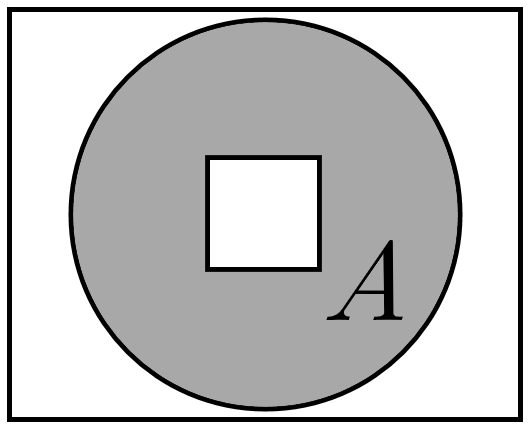
\includegraphics[width=1\textwidth]{Billeder/lufttvaer.png}
    \caption{\textit{Arealet som luften passerer gennem efter fordamperen}.}
    \label{fig:lufttvaer}
\end{figure}
\end{minipage}

Denne entalpi, samt luftens tryk på 1 bar, benyttes til at slå luftens temperatur op i \textit{EES}. Temperaturen efter fordamperen er fundet til:
\begin{equation}
    t_\text{b,beregnet} = \SI{3,30}{\celsius}
\end{equation}
Den beregnede afgangstemperatur er altså lavere end den gættede. Derfor ønskes det nu, gennem en iterativ proces, at finde frem til en mere korrekt værdi for luftens afgangtemperatur. Dette gøres ved at foretage samtlige udregninger i \ref{sec:dim_fordamper} med et nyt bud på luftens udgangstemperatur som vil resultere i sammenfaldende værdier for $t_\text{b}$ og $t_\text{b,beregnet}$.

Efter udførelse af denne iterative proces er der fundet frem til værdierne, som fremgår af tabellen nedenfor:
\begin{table}[H]
\centering
\begin{tabular}{|c|c|}
\hline
\multicolumn{2}{|c|}{\cellcolor[HTML]{C0C0C0}\textbf{Resultat af iterativ proces}} \\ \hline
$t_\text{b}$   & \SI{3,39}{\celsius}   \\ \hline
$\Phi_0$        & \SI{379}{W} \\ \hline
$U_\text{u}$    & \SI{28.6}{\frac{W}{m^2 \cdot K}} \\ \hline
\end{tabular}
\caption{\textit{Resultater for beregning af luftens afgangstemperatur, kuldeydelse og varmegennemgangstallet}.}
\end{table}

% ------------ Konklusion----------
\subsection{Delkonklusion (Alle)}
Kuldeydelsen ved de angivne forhold er, ud fra varmevekslerens dimensioner og de bestemte parametre, blevet beregnet til 379 W. Derfor kan det udledes, at denne varmeveksler lever op til den ønskede ydelse på 334 W. Kuldeydelsen er bestemt efter en iterativ proces, hvor afgangstemperaturen for luft er bestemt til \SI{3,39}{\celsius}.
Denne ydelse er ved forholdvis lav lufttemperatur inde i køleskabet. Dette betyder, at fordamperen vil være mere effektiv ved en højere lufttemperatur og trykket vil dermed også blive større på fordampersiden i køleanlægget. Dette gør systemet mere effektivt.
%------------------------------------------------------------
\end{document}
